\documentclass[10pt,a4paper]{scrartcl} 
\usepackage[left=1cm,right=1cm,top=1cm,bottom=1cm]{geometry} 
\usepackage[utf8]{inputenc} 
\usepackage[ngerman]{babel} 
\usepackage[most]{tcolorbox}
\usepackage[official]{eurosym}
\usepackage{amsmath}
\usepackage[bookmarks,bookmarksopen,bookmarksdepth=2]{hyperref}
\usepackage{cancel}
\usepackage{tabularx}
\usepackage{MnSymbol,wasysym}
\usepackage{tikz-timing}
\usepackage{tikz, pgfplots}
	\usepgfplotslibrary{groupplots}

\tikzset{
	timing/z/.style={color=blue},
	timing/l/.style={color=blue},
	timing/h/.style={color=blue}
}

\newtcbtheorem[no counter]{Theorem}{Definition}{
	enhanced,
	sharp corners,
	attach boxed title to top left={
		yshifttext=-1mm
	},
	colback=white,
	colframe=blue!75!black,
	fonttitle=\bfseries,
	boxed title style={
		sharp corners,
		size=small,
		colback=blue!75!black,
		colframe=blue!75!black,
	} 
}{thm}


\author{Levin Baumann}
\title{Digitaltechnik}

\begin{document}
	\maketitle
	\section{Begriffe}
	\begin{tabular}{r|l}
		digital & analog \\
		wertediskret & wertekontinuierlich\\
		$\Rightarrow$ zwischen zwei benachbarten gibt es \underline{keine} zwischenwerte & $\Rightarrow$ zwischen zwei beliebigen gibt es unendlich viele Zwischenwerte \\
		$ \Rightarrow $ endlich oder auch unendlich (aber abzählbar viele) & $ \Rightarrow $ Immer unendlich (und sogar überabzählbar) viele Werte \\
		meist zeitdiskret (\glqq getaktet\grqq) & zeitkontinuierlich \\
		$ \Rightarrow $ unsere heutigen Rechner arbeiten digital & $ \Rightarrow $ unsere Welt \glqq arbeitet\grqq\ analog
	\end{tabular}

\section{Codierung}

	\begin{Theorem}{}{fermat}
		Codierung ist die Darstellung von Informationen mit einem \glqq Alphabet\grqq.
	\end{Theorem}
		
	\begin{Theorem}{}{fermat}
		Alphabet ist eine \underline{endliche} Menge von Symbolen
	\end{Theorem}
	
	\textit{Anmerkung: Codierung ist immer mit Digitalisierung verbunden.} \\
	
	\subsection{Arten von Codierungen}
	\begin{itemize}
		\item Zeichencodierung
		\item Zahlencodierung (Text-, Bildbearbeitung,\dots)
		\item Verschlüssellung (\textit{Achtung:} Unterschied zu anderen Codierungen: Aus der codierten verschlüsselten Info sollen die meisten Menschen nicht auf die Ursprungsinfo schließen können)
		\item Signalcodierung
	\end{itemize}

	\subsection{Codierungen}
	\subsubsection{Zeichencodierung}
	\begin{itemize}
		\item ASCII: Alphabet besteht aus (ganzen) Zahlen von 0 bis 127
		\item ISO8859-x: Alphabet besteht aus 0\dots255
		\subitem -x: verschiedene Sprachräume
		\subitem -1: westeuropäisch
		\subitem -5: kyrillisch
		\subitem -7: griechisch
		\subitem -15: westeuropäisch inkl. \euro{}
		\item Unicode: Anspruch, alle (derzeitigen, künftigen, ehemaligen) Schriftsprachen abzudecken, auch Phantasiesprachen wie Klingonisch oder Elbisch
		\subitem UTF-8: 256 Zahlenwerte
		\subitem UTF-16: 65536 Zahlenwerte
		\subitem$ \rightarrow $ Zeichen werden als variabel lange Symbolfolgen dargestellt. Gesetztes MSB zeigt an, dass mindestens ein Folgesymbol folgt.
	\end{itemize}
	\subsubsection{Zahlencodierung}
	\paragraph{I. Abzählsysteme}
	\subparagraph{Fingerabzählsysteme}
	\begin{itemize}
		\item[] Alphabet = \{Finger\}
		\item[] Symbolwert (Finger) = 1
		\item[$ \ominus $] stark beschränkter Wertebereich von 0 bis 10
		\item[$ \ominus $] bis auf weiteres nur nicht-negative ganze Zahlen
		\item[$ \oplus $] extrem einfach und verständlich		
		\item[$ \oplus $] extrem einfache Addition und Subtraktion
		\item[$ \ominus $] Multiplikation und Divisionmit erhöhtem Aufwand
		\item[$ \oplus $] Immer verfügbar/\glqq zur Hand\grqq\
	\end{itemize}
	\subparagraph{Strichliste (einfache)}
	\begin{itemize}
		\item[] Alphabet = \{I\}
		\item[] Wert (I) = 1
		\item[$ \oplus $] unbeschränkter Wertebereich
		\item[$ \oplus $] Addition weiter einfach, Subtraktion braucht man eine Entfernungsmöglichkeit/Entwertungsmöglichkeit
		\item[$ \ominus $] Hilfsmittel (Schreibwerkzeug) notwendig
		\item[$ \ominus $] unübersichtlich darstellbarer Wertebereich bis etwa 10 (10 Symbole notiert)
	\end{itemize}
	\subparagraph{erweiterte Strichliste (\glqq Lattenzaunsystem \grqq)}
	\begin{itemize}
		\item[] Alphabet = {I, \cancel{\text{IIII}}}
		\item[] Wert ( I ) = 1
		\item[] Wert ( \cancel{\text{IIII}} ) = 5
		\item[] Regeln:Symbole müssen nach Wertigkeit sortiert notiert werden. Fünf einfache Striche müssen immer zu einem „Kombisymbol“ zusammengefasst werden.
		\item[$ \oplus/\ominus $] Addition etwas erschwert durch Sortieren und Zusammenfassen; Subtraktion zusätzlich erschwert durch Auflösen des Kombisymbols 
		\item[$ \oplus/\ominus $] etwas komplexer durch zweites Symbol und Sortierregel
		\item[$ \oplus/\ominus $] übersichtlich darstellbarer Wert bis etwa 50 erweitert
	\end{itemize}

	\subparagraph{römisches Zahlensystem}
	\begin{itemize}
		\item[] Alphabet = \{I, V, X, L, C, D, M\}
		\item[] Wert = \{1, 5, 10, 50, 100, 500, 1000\}
		\item[] Zusatzregel: Symbol kleinerer Wertigkeit darf vor einem Symbol größerer Wertigkeit notiert werden Sein Symbolwert wird dann subtrahiert, statt addiert. Mehr als drei gleiche Symbole sind nicht hintereinander erlaubt 
		\item[$ \oplus/\ominus $] übersichtlich darstellbarer Wertebereich bis etwa 10.000 (?)
		\item[$ \ominus $] beschränkter Wertebereich bis < 4000
		\item[$ \ominus $] recht hohe Komplexität, relativ geringe Verständlichkeit
		\item[$ \ominus $] extrem komplizierte Addition und Subtraktion
	\end{itemize}
	\paragraph{II. Stellenwertsysteme}
	\subparagraph{Dezimalsystem}
	\begin{itemize}
		\item[] Alphabet = \{0, 1, 2, 3, 4, 5, 6, 7, 8, 9\}
		\item[] Symbole werden auch Ziffern genannt
		\item[] Zahl ist notiert als Folge von Ziffern: z.B. 4711
		\item[] Ziffernwert = Symbolwert
		\item[] Ziffernwert (4) = 4
		\item[] Zahlenwert = Summe (Ziffernwert * Stellenwert) 
		\item[] Stellenwert (rechte Ziffer) = 1  
		\item[]Stellenwert wächst mit jeder Stelle nach links um Faktor 10
	\end{itemize}
	$$
	Wert(Z_{n-1} \dots Z_0) = \sum_{i=0}^{n-1}|Z_i|\cdot10^i
	$$
	\subparagraph{SWS zur Basis b}
	\begin{itemize}
		\item[] Alphabet enthält b Ziffern
		\item[] Alphabet beginnt bei Ziffer \glqq 0\grqq\ und endet bei Ziffer \glqq b-1\grqq\
	\end{itemize} 
	$$
		Wert(Z_{n-1} \dots Z_0) = \sum_{i=0}^{n-1}|Z_i| \cdot b^i
	$$
	$b_{EIN}$ mit $b>1$\\
	\textit{Anmerkung:} $b=1$ nicht sinnvoll, da im SWS zur Basis nur die 0 dargestelt werden könnte.
	\begin{itemize}
		\item[$ \oplus/\ominus $] gewisses \glqq Erstverständnis \grqq\/Lernaufwand ist nötig
		\item[$ \oplus/\ominus $] es gibt für jede Grundrechenart einVerfahren mit etwas erhöhter Komplexität, welches aber nach erstmaligem Lernaufwand doch relativ problemfrei realisierbar ist
		\item[$ \oplus/\ominus $] unbeschränkter Wertebereich
		\item[$ \oplus/\ominus $] Wertebereich bis etwa $b^10$ ist übersichtlich darstelbar
	\end{itemize}
	\subsubsection*{Umrechnung}
	\begin{itemize}
		\item Von Basis $b$ nach Basis $10$?
		\subitem $\Rightarrow$ Werteformel
		\item Von Basis $10$ nach Basis $ b $?
		\subitem $ \Rightarrow $ Werteformel umgekehrt
		\subitem $ \Rightarrow $ Ganzzahldivision
	\end{itemize}
	\begin{equation}
	\begin{split}
	{42}_{10} &= 101010\\	
	43:2 &= 21R0 = Z_0\\
	21:2 &= 10R1 = Z_1\\
	10:2 &= 5R0 = Z_2\\
	5:2  &= 2R1 = Z_3\\
	2:2  &= 1R0 =Z_4\\
	1:2	&= 0R1 = Z_5
	\end{split}
	\end{equation}
	Hinweis: Führende \glqq 0 \grqq\ können bei Zahlen im SWS beliebig hinzugefügt oder weggelassen werden. 
	allg: Umrechnung von Basis $b_1$ nach Basis $b_2$
	\begin{itemize}
		\item meist: von Basis $b_1$ nach $b_Z=10$ dann von $b_Z$ nach $b_2$
		\item theoretisch: Ganzzahldivision durch Zielbasis $b_2$, aber ausgeführt im SWS zur Ausgangsbasis $\Rightarrow$ Nicht praktikabel
	\end{itemize}
	Direkte Umrechnung:\\
	Falls $ b_1 = {b_2}^n $, dann entsprechen $n$ Ziffern zur Basis $ b_2 $ einer Ziffer zur Basis $ b_1 $ und es ist eine ziffern(block)weise Umrechnung.\\
	\\
	\underline{Bsp.:} $ b_1=2 $ und $ b_2=16 $\\
	$ \Rightarrow $ 4 Ziffern zur Basis $ 2 $ entsprechen einer Ziffer zur Basis $ 16 $.\\ \\
	
	\underline{Gängige Basen im SWS}\\
	$ b=10 $ \glqq Dezimalsystem\grqq\ $ \Rightarrow $ Mensch\\
	$ b=2 $ \glqq Binärsystem\grqq\/\glqq Dualsystem\grqq\ $ \Rightarrow $ Digitalrechner \\
	$ b=16 $ \glqq Hexadezimalsystem \grqq\ $ \Rightarrow $ Computernahe Darstellung von Zahlen
	\begin{itemize}
		\item weniger Stellen
		\item einfache Umrechnung
	\end{itemize}
	$ b=8 $ \glqq Oktalsystem\grqq\ $ \Rightarrow $ Computernahe Darstellung von Zahlen\\
	$ b=16 $ vs. $ b=8 $ nur \glqq normale\grqq\ Zahlen notwendig
	
	\subsubsection*{Hexadezimalsystem}
	\begin{tabular}{ccc}
		Wert & Ziffer & Binär\\
		0 & 0 & 0000\\
		1 & 1 & 0001\\
		2 & 2 & 0010\\
		3 & 3 & 0011\\
		4 & 4 & 0100\\
		5 & 5 & 0101\\
		6 & 6 & 0110\\
		7 & 7 & 0111\\
		8 & 8 & 1000\\
		9 & 9 & 1001\\
		10 & 10 & 1010\\
		11 & 11 & 1011\\
		12 & 12 & 1100\\
		13 & 13 & 1101\\
		14 & 14 & 1110\\
		15 & 15 & 1111\\
	\end{tabular}
\begin{minipage}[b]{0.7\textwidth}
	\centering
	BSP: $ABEF_{16}$
	$$
	\begin{array}{c|c|c|c}
	1010 & 1011 & 1110 & 1111
	\end{array}
	$$
	\\
	$$
	\begin{array}{c|c|c|c|ccc}
	0001&1001&0001&1100 & 0101_2 & = & 191C5_{16}\\
	1 & 9 & 1 & C & 5 & 
	\end{array}$$
\end{minipage}%
\\
\\
Falls $b_1^n = b_2^m$, dann entspricht ein Ziffernblock von $n$ Ziffern zur Basis $b_1$ einem Ziffernblock von $m$ Ziffern zur Basis $b_2$.
\\
$$
\begin{array}{rcl}
2^{3n} = 2^{4m} & \Rightarrow & n=4 \& m=3\\
				& \Rightarrow & \textrm{4 Ziffern zur Basis 8 entrsprechen}\\
				&             & \textrm{3 Ziffern zur Basis 16 entrsprechen}\\
				&             & \textrm{Problem: Tabelle hat } 2^{12} \textrm{ Zeilen}\\
\end{array}
$$

\subsubsection*{Einschränkungen aufheben}
\hspace*{2em}
auch negative Zahlen!
\\
Darstellung negativer Zahlen


%ToDo Rest aus Tablet übernehmen

\section{Signalkodierung}

\begin{Theorem}{}{fermat}
	Darstellung von abstrakten Informationen als Signalfolge. \\
	Signal: physisch messbare Größe.
\end{Theorem}

\subsection{mögliche Signalformen}
\begin{itemize}
	\renewcommand\labelitemi{--}
	
	\item elektrisch\\
		Spannung, Stromstärke, elektromagnetische Wellen, Ladung
	\item optisch\\
		Helligkeit, Farbe
	\item akustisch
		Lautstärke, Tonhöhe
	\item Druck
		hydraulisch, pneumatisch
\end{itemize}

\subsubsection*{in der Computertechnik relevant:}

\begin{list}{}{}
	\item[] optisch $\Rightarrow$ für netzwerkschnittstellen
	\item ekeltrisch $\Rightarrow$ insbesondere in der Digitaltechnik
	\subitem \textbf{vor allem:} Spannung (evtl. auch Stromstärke)\\
	\hspace*{2em}$\Rightarrow$ eher kleinere Spannungspegel in der Digitaltechnik
\end{list}

\subsubsection*{Strom Vs. Spannung}
\begin{figure}
	\centering
	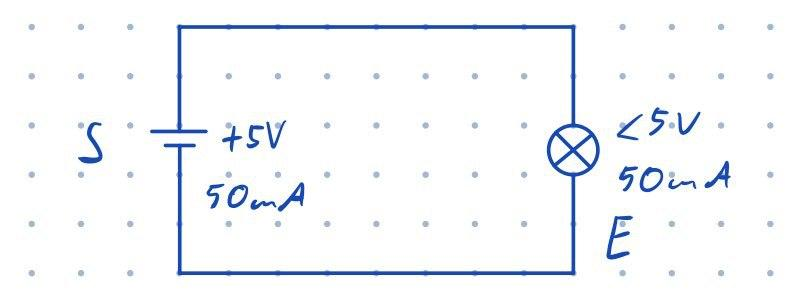
\includegraphics[width=0.5\linewidth]{img/strom_spannung_signale}
	\caption{Schaltplan mit Spannungsquelle und Glühbirne}
	\label{abb:schaltplan}
\end{figure}

\begin{tabularx}{\linewidth}{r X}
	Spannung: & Verringert sich beim E durch Spannungsfall auf der Leitung, wird verändert durch Störungen von außen (\glqq Übersprechen\grqq\, elektromagnetische Einstrahlungen)\\
	Strom: & Kaum davon betroffen; Stromstärke verändert sich im geschlossenen Stromkreis nicht.\\
\end{tabularx}
\\
Nachteil Strom: hoher Energieaufwand, große Wärmeentwicklung\\
\hspace*{2em}$\Rightarrow$ deshalb Spannung statt Strom bei den meisten Computerschnittstellen verwandt.
\\

\subsection*{typische Spannungspegel:}
\hspace*{3em}
$ \left.  \begin{array}{ccc}
0 & \hat{=} & 0V \\
1 & \hat{=} & 5V
\end{array} \right\rbrace 
$ TTL-Pegel
\\\\
\glqq Transistor-Transistor-Logic\grqq \\
\hspace*{2em} $\Rightarrow$ \glqq erfunden\grqq um 1960 von TI (TexasInstruments)

\subsubsection*{große vs. kleine Spannungspegel}

\begin{itemize}
	\item[$\bigominus$] größere sind stromanfällig bei kleineren Spannungen
	\item[$\bigoplus$] viel weniger Energieaufwand bei kleinen Spannungen, also auch weniger Wärmeentwicklung
	\item[$\bigoplus$] weniger Störauswrkungen bei kleineren Spannungen
	\item[$\bigoplus$] schnelleres Spannungswechseln bei kleinen Spannungshüben möglich
\end{itemize}

\subsection{Umsetzung von Bitfolgen in Spannungspegelfolgen}
\hspace*{2em} meist getaktet, d.h. festes Zeitraster für die Bitfolge, d.h. jedes Bit braucht eine konstante, gleichlange zeitdauer



\subsubsection*{4 Verfahren (1-4) und 4 Eigenschaften(a-d)}

\begin{enumerate}
	\item NRZ (Non-Return-to-zero)\\
		Während der gesamten Schrittdauer wird der Pegel angegegt, welcher dem zu übertragenen Bitwert entspricht
	\item RZ (Return-to-Zero)
		Jeder Schritt wird in zwei Schrittzeithälften eingeteilt. Während der ersten Hälfte wird der Pegel eingenommen, welcher den zu übertragenden Bitwert entspricht und während der zweiten Hälfte immer der \glqq0\grqq\-Pegel.
		\subitem TRG bei RZ: Bei jeder \glqq1\grqq\ möglich, dann bei einer \glqq1\grqq\ zu Beginn und in der Mitte der Schrittzeit ein Pegelwechsel stattfindet
	\item AMI (Alternate Mark Inversion)\\
		Ähnlich NRZ mit single-ended Pegeln, d.h. \glqq0\grqq\ wird immer mit $0V$ (während der gesamten Schrittzeit) übertragen, aber \glqq1\grqq\ abwechselnd mit z.B. $+5V$ und $-5V$ (während der gesamten Schrittzeit)
		\subitem GFS bei AMI: nachjeder 2. \glqq1\grqq: In der Praxis ist der GS-Anteil nach der ungeraden \glqq1\grqq\ vernachlässigbar (bei langer Übertragungszeit und vielen übertragenen \glqq1\grqq), also praktisch immer GSF.
		\subitem TRG bei AMI: bei jeder \glqq1\grqq\ nur bei langer Folge von \glqq0\grqq\ keine TRG möglich
	\item Manchester\\
		Bitwert wird über Spannungswechsel in der Mitte der Schrittzeit dargestellt, z.B. steigende Flanke $\hat{=}$ \glqq1\grqq und fallende Flanke $\hat{=}$ \glqq 0 \grqq.\\
		ggf. ist ein weiterer Spannungswechsel zu Beginn der Schrittzeit notwendig, um den nachfogenden (inhaltsführenden) Spannungswechsel durchführen zu können.
		\subitem TRG bei Manchester: bei jedem Schritt möglich, da immer Regelwechsel in der Mitte der Schrittzeit.
		\subitem GFS bei Manchester: immer, da sich die Pegel in erster und zweiter Schrittzeithälfte gegenseitig ausgleichen
		\subitem SSH bei Manchester: optimal, da \glqq nur \grqq 2 Pegel
\end{enumerate}

\begin{enumerate}
	\item[a)] TRG (Taktrückgewinnung)\\
		Möglichkeit, nur aus dem übertragenen Datensignal eine Resynchronisierung biem Empfänger auf den Takt des Senders zu machen
	
	\item[b)] GSF (Gleichspannungs-/stromfreiheit)\\
		Motivation: Einsparung der Masseleitung. Im zeitlichen Mittel liegen auf der Signalleitung 0V an.\\
		Ziel: Anhand des mittleren Signalpegels soll der Massepegel \glqq errechnet\grqq\ werden.\\
		\subitem -Vermeidung einer Potentialverschiebung beim E.
		\subitem -Pseudoargument: keine Energieübertragung beim vom S zum E.\\
		Grundvoraussetzung: symmetrische Pegel statt single-ended. \\
		z.B. $1V \hat{=} +5v$ und $0 \hat{=} -5V$\\
		dann: GSF bei NRZ: falls \#\glqq0\grqq\ = \#\glqq1\grqq\ (bzw. \glqq1\grqq\ und \glqq0\grqq\ im Datenstrom gleichverteilt)\\\\
		Bei den meisten Anwendungs-, Zeichen- und Zahlencodierungen kann keine Gleichverteilung angenommen werden. Ausnahme: Verschlüsselung und Kompression.
	\item[c)] SSH (Störsicherheit)\\
		(Un-)Anfälligkeit eines Verfahrens ggü. Störungen, welche durch Spannungsschwankungen auf der Leitung verursacht werden.\\
		$\Rightarrow$ direkt abhängig von der Anzahl der verwendeten Pegel, welche auf einen vorgegebenen Potentialbereich verteilt werden müssen (und so natürlich auch beim Empfänger voneinander unterschieden werden müssen)\\
		SSH bei AMI: schlecht, da 3 Pegel\\
		SSH bei NRZ und RZ: gut, da \glqq nur\grqq\ 2 Pegel (und weniger Pegel geht nicht \smiley{})
\end{enumerate}

\begin{figure}[h]
	\centering
	\begin{tikztimingtable}[timing/slope=0, scale=4]
		Data    	&  \\
		NRZ     	& ZHZHZHZZZZHHHHH \\
		RZ 		    & ZhzZhzZhzZZZZhzhzhzhzhz\\
		AMI        	& ZHZLZHZZZZLHLHL \\
		Manchester 	& hzzhhzzhhzzhhzhzhzhzzhzhzhzhzh\\
		\extracode
		\makeatletter
		\tikzset{
			timing/z/.style={color=red},
			timing/l/.style={color=red},
			timing/h/.style={color=red}
		}
		\begin{pgfonlayer}{background}
			\foreach [count=\x] \b in {0,1,0,1,0,1,0,0,0,0,1,1,1,1,1} {
				\node [below,font=\sffamily\bfseries\tiny,inner ysep=2pt] at (\x-.5,.5) {\b};
			}
			\vertlines[help lines, black]{}
			\horlines[black,yshift=1.25mm]{}
		\end{pgfonlayer}
	\end{tikztimingtable}
\caption{Pegelgraphen der einzelnen Verfahren}
\end{figure}

\subsubsection*{Bandbreitenbedarf, bandbreitenbegrenzte Übertragungskanäle}
	Nyquist-Theorem: Über einen Übertragungskanal mit beschränkter Bandbreite kann maximal mit der Schrittrate übertragen werden, welche der doppelten Bandbreite entspricht.\\
	BBB (Bandbreitenbedarf): notwendige Bandbreite für ein bestimmtes Signalcodierungsverfahren bei einem 

\end{document}